\documentclass[12pt,a4paper]{report}

\usepackage[utf8]{inputenc}
\usepackage[T1]{fontenc}
\usepackage[main=english]{babel}
\usepackage{lmodern}
\usepackage{geometry}
\usepackage{setspace}
\usepackage{graphicx}
\usepackage{float}
\usepackage{booktabs}
\usepackage{tabularx}
\usepackage{longtable}
\usepackage{array}
\usepackage{enumitem}
\usepackage{xcolor}
\usepackage{amsmath}
\usepackage{amssymb}
\usepackage{tikz}
\usepackage{pgfplots}
\usetikzlibrary{positioning}
\usepackage{listings}
\usepackage{caption}
\usepackage{subcaption}
\usepackage{fancyhdr}
\usepackage[hidelinks]{hyperref}
\usepackage[toc,page]{appendix}
\usepackage{titlesec}
\usepackage{indentfirst}
\usepackage{parskip}

\geometry{left=2.5cm,right=2.5cm,top=2.5cm,bottom=2.5cm,headheight=2.5cm}
\onehalfspacing
\setlength{\parindent}{0.75cm}
\setcounter{secnumdepth}{3}
\setcounter{tocdepth}{3}

\newcommand{\HRule}{\rule{\linewidth}{0.5mm}}

\pagestyle{fancy}
\fancyhf{}
\rhead{\rightmark}
\lfoot{\leftmark}
\rfoot{Page \thepage}
\renewcommand{\headrulewidth}{1pt}
\renewcommand{\footrulewidth}{1pt}

\lstdefinestyle{code}{
    basicstyle=\ttfamily\small,
    breaklines=true,
    frame=single,
    numbers=left,
    numberstyle=\tiny,
    keywordstyle=\color{blue},
    commentstyle=\color{gray},
    stringstyle=\color{teal},
    captionpos=b
}
\lstset{style=code}

\pgfplotsset{compat=1.18}

\begin{document}

% =========================================================
% Cover page
% =========================================================
\begin{titlepage}
    \begin{center}
        \MakeUppercase{Republic of Tunisia}\\
        \vspace{0.1cm}
        \MakeUppercase{Ministry of Higher Education and Scientific Research}\\
        \vspace{0.1cm}
        \MakeUppercase{University of Carthage}\\
        \vspace{0.2cm}
        \textbf{National Engineering School of Carthage}\\
        \vspace{0.8cm}

        \IfFileExists{Images/enicarthage.png}{
            \includegraphics[width=0.28\linewidth]{Images/enicarthage.png}
        }{
            \fbox{\parbox[c][3cm][c]{6cm}{\centering Institution logo}}
        }

        \vspace{0.6cm}
        \textbf{\large Computer Science Department}\\
        \vspace{0.3cm}
        \Large Capstone Project Report\\
        \vspace{0.4cm}

        \HRule\\[0.35cm]
        \Large
        \textbf{Design and Implementation of an On-Chain Trading Platform on Solana}\\[0.15cm]
        \large Opportunity Detection, Atomic Execution, Risk Protection, and Artificial Intelligence Signals
        \\[0.25cm]
        \HRule

        \vspace{0.5cm}
        \large Submitted by:\\
        \textbf{Name Surname}\\
        \vspace{0.4cm}

        \renewcommand{\arraystretch}{1.2}
        \begin{tabular}{@{}ll@{}}
            Academic supervisor: & Mr./Mrs. Name Surname \\
            Professional supervisor: & Mr./Mrs. Name Surname \\
            Host organization: & Company / Laboratory name \\
        \end{tabular}

        \vfill

        \begin{large}
            \textbf{Academic Year}\\
            2025--2026
        \end{large}
    \end{center}
\end{titlepage}

% =========================================================
% Signatures
% =========================================================
\thispagestyle{empty}

\begin{center}
  \begin{tikzpicture}
    \draw[rounded corners=20pt] (0,0) rectangle (16,9);
    \node at (8,8) {\textbf{Professional Supervisor}};
    \node at (8,7) {Mrs. Wiem LAGHA};
    \node[anchor=west] at (10,3.5) {\textbf{Signature}};
  \end{tikzpicture}
\end{center}

\begin{center}
  \begin{tikzpicture}
    \draw[rounded corners=20pt] (0,0) rectangle (16,9);
    \node at (8,8) {\textbf{Academic Supervisors}};
    \node at (3,7) {Dr. Amor GUEDDENA};
    \node at (13,7) {Dr. Haythem GHAZOUANI};
    \node[anchor=west] at (12,3.5) {\textbf{Signature}};
    \node[anchor=west] at (12,2.5) {};
    \node[anchor=west] at (2,3.5) {\textbf{Signature}};
    \node[anchor=west] at (2,2.5) {};
  \end{tikzpicture}
\end{center}

\newpage

% =========================================================
% Dedication
% =========================================================
\chapter*{Dedication}
\addcontentsline{toc}{chapter}{Dedication}
\rhead{Dedication}

\vspace*{\fill}

\newpage

% =========================================================
% Acknowledgements
% =========================================================
\chapter*{Acknowledgements}
\addcontentsline{toc}{chapter}{Acknowledgements}
\rhead{Acknowledgements}

I would first like to express my sincere gratitude to my academic supervisor for the guidance, feedback, and support provided throughout this project. This supervision helped me structure the work, clarify the technical objectives, and maintain a rigorous engineering approach.

I would also like to thank my professional supervisor and the team that supported me during the development of this project. The technical discussions, architectural reviews, and exchanges around the real constraints of on-chain trading contributed significantly to the evolution of the proposed solution.

Finally, I would like to thank my family, friends, and everyone who encouraged me during this period. Their support was valuable both during difficult phases and during the most rewarding stages of the project.

\newpage

% =========================================================
% Tables
% =========================================================
\tableofcontents
\listoftables
\listoffigures
\newpage

% =========================================================
% Acronyms
% =========================================================
\chapter*{List of Acronyms}
\addcontentsline{toc}{chapter}{List of Acronyms}
\rhead{List of Acronyms}

\begin{itemize}
    \item \textbf{AMM}: Automated Market Maker.
    \item \textbf{API}: Application Programming Interface.
    \item \textbf{CPI}: Cross-Program Invocation.
    \item \textbf{DeFi}: Decentralized Finance.
    \item \textbf{DEX}: Decentralized Exchange.
    \item \textbf{GRU}: Gated Recurrent Unit.
    \item \textbf{AI}: Artificial Intelligence.
    \item \textbf{IDL}: Interface Description Language.
    \item \textbf{LLM}: Large Language Model.
    \item \textbf{MEV}: Maximal Extractable Value.
    \item \textbf{PDA}: Program Derived Address.
    \item \textbf{RPC}: Remote Procedure Call.
    \item \textbf{SPL}: Solana Program Library.
    \item \textbf{TTL}: Time To Live.
    \item \textbf{WebSocket}: Real-time bidirectional communication protocol.
\end{itemize}

\newpage

% =========================================================
% General introduction
% =========================================================
\chapter*{General Introduction}
\addcontentsline{toc}{chapter}{General Introduction}
\rhead{General Introduction}

Decentralized finance has deeply changed the way digital assets can be exchanged, borrowed, lent, and used in automated strategies. Unlike centralized platforms, on-chain protocols expose their state, liquidity reserves, and transactions directly through the blockchain. This transparency makes it possible to build systems that continuously monitor markets, detect opportunities, and automatically execute transactions.

However, this openness also introduces major technical constraints. An on-chain trading system must handle RPC latency, transaction fees, slippage, competition between bots, MEV risks, malicious tokens, manipulated pools, and atomicity requirements for specific strategies. An opportunity that appears profitable in theory can become a loss if it is executed too late, if fees are underestimated, or if the target token behaves maliciously.

In this context, this project focuses on the design and implementation of an on-chain trading platform on Solana. Solana was chosen because of its low transaction costs, high throughput, and active DeFi ecosystem. The developed system combines a TypeScript backend, Anchor programs deployed on DevNet, a Python artificial intelligence server, a Redis cache layer, and a multi-user architecture that manages several trading configurations.

The project addresses the following problem: how can we design a platform capable of detecting, filtering, and executing on-chain trading opportunities while maintaining a level of security, reliability, and observability suitable for a decentralized environment?

To answer this problem, the work is structured around four main contributions. First, an opportunity discovery layer identifies arbitrage, liquidation, yield, and directional opportunities. Second, a routing component separates opportunities requiring fast atomic execution from opportunities that require a more cautious path. Third, a multi-stage safety pipeline limits exposure to risky tokens and abnormal behavior. Finally, a decision model aggregates several AI signals in order to better control decisions involving user capital.

This report is organized into seven chapters. Chapter 1 presents the general project framework and problem statement. Chapter 2 introduces the state of the art related to on-chain trading, flash loans, DeFi risks, and AI-based signals. Chapter 3 describes the functional and non-functional requirements. Chapter 4 presents the global architecture of the system. Chapter 5 details the design and implementation of the main components. Chapter 6 focuses on artificial intelligence signals and their integration. Finally, Chapter 7 presents the experimental setup, evaluation metrics, discussion, limitations, and perspectives.

% =========================================================
% Chapter 1
% =========================================================
\chapter{General Project Framework}
\label{chap:framework}
\rhead{General Project Framework}

\section{Introduction}

This chapter introduces the general framework of the project. It presents the professional environment in which the work was carried out, the technological context, the academic scope, the problem statement, the objectives, and the adopted methodology. It situates the work in an environment combining blockchain, decentralized finance, automated execution, and artificial intelligence.

\section{Professional Framework}

The development of this project took place within a professional context centered on technological innovation and applied research. Since the subject combines blockchain engineering, artificial intelligence, software architecture, and financial automation, the host environment played an important role in shaping the technical direction of the work. This section presents the host company, its innovation-oriented structure, and the initial training framework that supported the project.

\subsection{Host Company}

Talan is an international consulting and technology group founded in 2002 by Mehdi Houas, Eric Benamou, and Philippe Cassoulat. The company supports organizations in their digital transformation by combining management consulting, information systems expertise, data, artificial intelligence, cloud, and emerging technologies. According to the group's public presentation, Talan now operates internationally and brings together more than 7,000 employees across multiple countries and continents \cite{talanWho}.

The group works with clients in strategic sectors such as banking and financial services, energy, transport, public services, retail, luxury, and healthcare. Its positioning is based on the ability to transform technological innovation into concrete business value. This makes it a relevant environment for a project involving decentralized finance and automated decision systems, since such a subject requires both engineering rigor and an understanding of financial use cases.

Talan Tunisie represents one of the group's important technology hubs. It contributes to the design and implementation of software solutions for international clients while also participating in innovation-oriented projects. The Tunisian branch provides an environment where engineering students can work on applied topics involving modern software architectures, data-driven systems, blockchain, and artificial intelligence.

\subsection{Talan Innovation Factory}

The Talan Innovation Factory is part of the group's broader innovation strategy. Its role is to explore emerging technologies, prototype new solutions, and support projects that may later become industrial or client-facing assets. The initiative focuses on domains such as artificial intelligence, data intelligence, blockchain, extended reality, and other advanced digital technologies \cite{talanSummer}.

This innovation framework is particularly aligned with the subject of this project. The trading platform developed in this work is not a simple application layer; it combines on-chain programs, event-driven backend services, AI signals, risk controls, and user-facing monitoring. Such a combination requires experimentation, fast iteration, and the ability to evaluate technical trade-offs before considering production hardening.

Within this context, the Innovation Factory provides a setting where exploratory engineering can be connected to practical implementation. It encourages the study of recent technologies while maintaining a project-oriented approach. For this project, that means testing the feasibility of on-chain trading strategies on Solana DevNet, designing protection mechanisms, and integrating AI signals in a controlled and measurable way.

\subsection{Bootcamp}

Before the main project implementation phase, interns take part in an introductory training program designed to build a common technical foundation. This bootcamp exposes participants to several advanced topics and encourages autonomous learning, technical presentations, teamwork, and rapid prototyping.

The training program generally covers subjects related to artificial intelligence, generative AI, natural language processing, computer vision, blockchain, decentralized applications, and other emerging technologies. Its purpose is not only to introduce tools, but also to develop the ability to analyze a problem, choose an appropriate technical approach, and communicate results clearly.

For this project, the bootcamp was useful because it provided a broader view of the technologies involved in the final solution. The blockchain sessions helped frame the Solana and smart contract aspects, while the AI-oriented sessions supported the integration of predictive and sentiment-based signals. This initial preparation also helped establish the engineering habits required for the rest of the work: documentation, experimentation, validation, and iterative improvement.

\section{Technological Context}

Decentralized finance, or DeFi, refers to a set of financial protocols built on public blockchains. These protocols allow users to exchange assets, borrow, lend, provide liquidity, or execute complex strategies without relying on a centralized intermediary. Smart contracts replace part of the logic traditionally handled by financial institutions.

In such an environment, markets are continuously accessible and their state can be read directly from the blockchain. This property is particularly useful for automated systems, because it enables the development of bots capable of observing pool reserves, prices, lending positions, and wallet activity.

Solana stands out in this ecosystem because of its high throughput and low transaction fees. These characteristics make it suitable for strategies that are sensitive to latency. However, network performance does not eliminate on-chain execution risks. The system must still account for transaction confirmation, RPC availability, liquidity variation, and competition between market participants.

From an engineering perspective, this context creates a system design problem rather than a simple trading problem. The bot must interact with blockchain accounts, construct valid transactions, estimate execution costs, and handle asynchronous events. At the same time, it must protect user capital from unsafe opportunities. This dual requirement explains the layered architecture adopted in this project: one layer detects opportunities, another verifies them, another protects capital, and a final layer executes transactions.

\section{Academic and Professional Scope}

This project is positioned at the intersection of academic research and applied software engineering. From an academic perspective, it studies how an automated on-chain system can combine deterministic trading logic, smart contract execution, risk filters, and artificial intelligence signals. From a professional perspective, it aims to produce a working prototype with clear components, tests, and deployment assumptions.

The work does not aim to deploy a production trading system directly on MainNet. Instead, it focuses on validating the architecture in a controlled environment. Solana DevNet is used to deploy test programs, create artificial pools, simulate arbitrage gaps, and execute transactions without exposing real funds. This choice makes it possible to test the technical feasibility of the approach while keeping the experimentation safe.

The project also prepares several components for future hardening. The use of per-user vaults, event-driven orchestration, API-based configuration, and protection rules reflects a design that can later evolve toward a more robust platform.

\section{Problem Statement}

Building an on-chain trading bot is not limited to detecting a price difference. An opportunity must be profitable after fees, executable in the current market state, protected against malicious tokens, and routed through an execution path adapted to its risk.

In practice, several constraints interact at the same time. A profitable arbitrage may disappear before the transaction is confirmed. A token may appear liquid but contain unsafe properties. A model may predict a favorable direction while market conditions change abruptly. A user may configure a high-risk strategy without enough capital protection. These cases show that opportunity detection must be separated from execution decision-making.

The central problem can therefore be formulated as follows:

\begin{quote}
How can we design a modular architecture capable of detecting on-chain trading opportunities, filtering them according to safety criteria, and executing them reliably and observably on Solana?
\end{quote}

This problem raises several sub-questions:
\begin{itemize}
    \item how to distinguish opportunities requiring atomic execution from those that can be evaluated more slowly;
    \item how to integrate protections that are independent from the trading strategy;
    \item how to use AI without confusing predictive signals with uncontrolled automatic decisions;
    \item how to isolate user funds in a multi-user architecture;
    \item how to measure system performance and robustness.
\end{itemize}

The proposed solution answers these questions through modular decomposition. Each component has a limited responsibility: detectors identify candidates, the router classifies them, the safety pipeline checks token and opportunity risks, the protection layer enforces capital rules, and the execution layer constructs the final transaction.

\section{Project Objectives}

The main objective is to design and implement a modular on-chain trading platform on Solana. The system must support the detection, validation, routing, and execution of opportunities in a controlled DevNet environment, while preparing several components for a possible future migration to MainNet.

The specific objectives are:
\begin{enumerate}
    \item set up a backend infrastructure capable of communicating with Solana, Redis, and an AI server;
    \item implement opportunity detectors for arbitrage, liquidation, yield, and directional signals;
    \item design a router that separates the fast path from the slow path;
    \item integrate an S1--S4 safety pipeline;
    \item develop a protection layer independent from the detectors;
    \item build atomic Solana transactions for fast execution strategies;
    \item deploy Anchor programs for the AMM, flash loan, vault, and lending logic;
    \item integrate AI signals into a decision model;
    \item expose a multi-user platform with an API, WebSockets, and dynamic configuration propagation.
\end{enumerate}

\section{Methodology}

The adopted methodology was inspired by the Scrum agile framework. This choice was motivated by the exploratory nature of the project. The platform combines several complex domains, including blockchain programming, decentralized finance, artificial intelligence, backend engineering, and risk management. A strictly sequential methodology would have been difficult to apply because several technical choices had to be validated progressively through experimentation.

The work was therefore organized into a research sprint followed by implementation sprints. Each sprint had a clear objective, a set of deliverables, and a validation phase. At the end of each sprint, the implemented components were tested and the next tasks were adjusted according to the technical results obtained. This iterative organization made it possible to reduce uncertainty, especially for the parts related to Solana transactions, Anchor programs, and AI signal integration.

\subsection{Scrum Roles}

The project was carried out individually, but the Scrum roles were adapted to the academic context. The student acted as the development team and was responsible for analysis, implementation, testing, and documentation. The academic supervisor played the role of product owner from an academic perspective by validating the relevance of the objectives and the structure of the report. The professional supervisor acted as a technical stakeholder by providing feedback on architectural choices, feasibility, and engineering quality.

\subsection{Sprint Organization}

The project was organized into Sprint 0 and four implementation sprints. Sprint 0 was dedicated to research and technical framing, while the following sprints focused on building the platform incrementally.

\begin{table}[H]
\centering
\begin{tabularx}{\textwidth}{lX X}
\toprule
\textbf{Sprint} & \textbf{Objective} & \textbf{Main Deliverables} \\
\midrule
Sprint 0 & Research and framing & Study of Solana, DeFi trading, AMMs, flash loans, MEV risks, Anchor, and AI signals. Definition of the initial architecture and backlog. \\
Sprint 1 & Infrastructure and DevNet environment & TypeScript backend setup, Solana RPC connection, wallet loading, Redis cache, DevNet tokens, AMM pools, and configuration files. \\
Sprint 2 & Opportunity discovery and safety & Arbitrage, liquidation, and yield detectors; safety pipeline S1--S4; token risk checks; cached scores; first unit tests. \\
Sprint 3 & Execution and protection & Transaction builders, flash loan execution, vault-based execution, ProtectionManager, slippage guard, drawdown rules, and auto-pause. \\
Sprint 4 & AI, orchestration, and multi-user platform & Python AI server, DecisionModel, graph-based orchestration, per-user lanes, API, WebSockets, and end-to-end tests. \\
\bottomrule
\end{tabularx}
\caption{Sprint organization}
\label{tab:sprints}
\end{table}

\subsection{Product Backlog}

The product backlog was used to organize the main features of the platform. Items were prioritized according to dependency order and project risk. Core infrastructure and on-chain execution were treated as high priority because the other components depend on them. AI and multi-user features were added after the execution and protection layers became stable.

\begin{longtable}{p{1.4cm}p{4.6cm}p{6.1cm}p{2cm}}
\toprule
\textbf{ID} & \textbf{Backlog item} & \textbf{Description} & \textbf{Priority} \\
\midrule
P1 & Solana backend infrastructure & Connect to RPC, load wallet, read configuration, initialize logger and cache. & High \\
P2 & DevNet simulation environment & Create test tokens, pools, and controlled liquidity scenarios. & High \\
P3 & AMM Anchor program & Implement swap and liquidity instructions for controlled testing. & High \\
P4 & Flash loan program & Implement atomic borrow and repay logic for arbitrage execution. & High \\
P5 & Arbitrage detector & Detect triangular arbitrage opportunities from pool reserves. & High \\
P6 & Liquidation detector & Detect undercollateralized positions from the lending program. & Medium \\
P7 & Safety pipeline S1--S4 & Reject risky tokens and abnormal opportunities before execution. & High \\
P8 & ProtectionManager & Apply slippage, drawdown, trading hours, and auto-pause rules. & High \\
P9 & Vault program & Isolate user funds through a dedicated PDA. & High \\
P10 & AI server & Provide sentiment, regime, volatility, and direction signals. & Medium \\
P11 & DecisionModel & Fuse AI signals into a single score for slow-path decisions. & Medium \\
P12 & Graph orchestration & Replace a simple sequential loop with event-driven graph execution. & Medium \\
P13 & Multi-user API & Manage users, configurations, statuses, and WebSocket updates. & Medium \\
P14 & Testing and evaluation & Add unit, integration, and end-to-end tests for the full pipeline. & High \\
\bottomrule
\caption{Product backlog}
\label{tab:backlog}
\end{longtable}

This Scrum-inspired approach helped keep the project manageable. Each sprint produced a usable increment, while the backlog ensured that the most critical technical risks were addressed early.

\section{Conclusion}

This chapter presented the context, challenges, and objectives of the project. The work belongs to a domain where execution performance must be balanced with safety and robustness. The next chapter presents the state of the art required to understand the concepts used in the proposed solution.

% =========================================================
% Chapter 2
% =========================================================
\chapter{State of the Art}
\label{chap:state_of_art}
\rhead{State of the Art}

\section{Introduction}

This chapter presents the main concepts required to understand the project. It covers on-chain trading strategies, atomic execution mechanisms, major risks encountered in DeFi, and the use of artificial intelligence signals in a decision-making system.

\section{On-Chain Trading and Automated Market Makers}

Automated Market Makers replace the traditional order book with a mathematical function linking the reserves of two assets. In a constant-product model, the product of the reserves remains approximately constant:

\begin{equation}
    x \cdot y = k
\end{equation}

where $x$ and $y$ represent the reserves of the two tokens, and $k$ is a constant. When a trader swaps one asset for another, reserves change and the implicit price evolves. This mechanism creates price differences between pools, especially when pools are not immediately rebalanced.

An arbitrage bot attempts to exploit these differences. In triangular arbitrage, the bot performs a sequence of swaps between three assets. If the final amount is greater than the initial amount after fees, the operation is profitable.

The constant-product model also implies that the execution price depends on trade size. A large swap changes the pool reserves significantly and therefore produces slippage. For this reason, an opportunity detector must not only compare displayed prices, but also simulate the expected output amount for a given input size. This is especially important for on-chain trading bots, because a theoretical price gap can disappear once the trade size and fees are considered.

In this project, AMM pools are reproduced on Solana DevNet through a dedicated Anchor program. This makes it possible to control reserves, create test price gaps, and validate the arbitrage logic in a deterministic environment before considering real liquidity sources.

\section{Arbitrage, Liquidation, and Yield}

Arbitrage consists in exploiting a price difference between several markets. On Solana, it can be executed through successive swaps in AMM pools. The main difficulty is that the opportunity can disappear quickly, since other actors observe the same price gaps.

Liquidation concerns lending protocols. When a borrower becomes undercollateralized, a liquidator can repay part of the debt and receive part of the collateral with a bonus. This strategy requires reliable reading of position states and fast execution when the health ratio becomes insufficient.

Yield strategies aim to identify opportunities where capital can be allocated to protocols or pools offering attractive returns. Unlike arbitrage, these decisions are generally less atomic and involve user capital. Therefore, they require additional checks.

These three families of opportunities do not have the same execution requirements. Arbitrage is highly sensitive to latency and usually requires immediate execution. Liquidation is also time-sensitive because several liquidators may compete for the same position. Yield and directional strategies are less urgent but expose user capital for a longer period. The architecture therefore separates fast opportunities from slow opportunities instead of applying the same decision process to all strategies.

\begin{table}[H]
\centering
\begin{tabularx}{\textwidth}{lX X}
\toprule
\textbf{Opportunity} & \textbf{Main constraint} & \textbf{Preferred path} \\
\midrule
Arbitrage & Very low latency and atomic execution. & Fast path \\
Liquidation & Fast reaction to position health changes. & Fast path \\
Yield & Capital allocation and risk control. & Slow path \\
Directional AI signal & Prediction confidence and protection rules. & Slow path \\
\bottomrule
\end{tabularx}
\caption{Opportunity types and execution paths}
\label{tab:opp_paths}
\end{table}

\section{Flash Loans and Atomicity}

A flash loan allows a user to borrow an asset without collateral, provided that the loan is repaid within the same transaction. This mechanism is useful for strategies that temporarily require significant capital without locking that capital permanently.

Atomicity is essential: if the borrow, swaps, and repayment cannot all be executed, the whole transaction fails. The bot therefore avoids keeping an open debt or an inconsistent intermediate position.

In this project, the fast path relies on this logic. An arbitrage transaction can follow the sequence below:

\begin{center}
\texttt{flash\_borrow} $\rightarrow$ \texttt{swap 1} $\rightarrow$ \texttt{swap 2} $\rightarrow$ \texttt{swap 3} $\rightarrow$ \texttt{flash\_repay}
\end{center}

The advantage of this design is that the bot does not need to permanently hold the full amount required for the arbitrage. However, it also means that the transaction builder must be precise. All accounts, instructions, token transfers, and repayment constraints must be included in the same transaction. If one instruction is missing or ordered incorrectly, the transaction must fail.

This requirement influenced the implementation of the execution layer. The transaction builder is separated from the detector so that opportunity discovery remains independent from low-level Solana transaction construction.

\section{Risks Specific to DeFi}

\subsection{MEV}

MEV refers to the value that an actor can extract by observing, reordering, or inserting transactions. In a trading context, a bot can be front-run by another actor or suffer a sandwich attack. Even when the opportunity is real, the execution environment can reduce or cancel profitability.

For a DevNet prototype, MEV is mainly studied as an architectural risk rather than fully reproduced. The system nevertheless includes concepts that prepare future hardening, such as fee-aware profit checks, slippage limits, and a dedicated transaction submission layer.

\subsection{Honeypots and Malicious Tokens}

A honeypot is a token or pool that allows buying but prevents selling, or applies unfavorable rules at exit time. Rug pulls and misconfigured tokens can also cause capital loss. A trading system must therefore verify on-chain token properties before committing funds.

The project addresses this issue through a multi-level safety pipeline. Basic rules reject suspicious token properties early, while deeper checks attempt to identify abnormal behavior. This approach reduces the probability of executing a transaction against a malicious or manipulated asset.

\subsection{Slippage and Fees}

Slippage is the difference between the expected price and the actual execution price. It increases when the order size is large relative to available liquidity. Network fees, priority fees, and protocol fees must also be integrated into profitability calculations.

Ignoring fees is one of the most common causes of false opportunities. A small arbitrage margin can be fully consumed by network fees or priority fees. For this reason, the project includes a fee-aware guard that compares expected profit against estimated execution cost before submitting a transaction.

\section{AI and Predictive Signals}

Artificial intelligence can provide useful signals, but it does not guarantee profitable decisions. In a financial environment, models can be sensitive to noise, regime changes, and data quality. It is therefore preferable to use them as components of a decision model rather than as a single source of truth.

The signals considered in this project include:
\begin{itemize}
    \item social or news sentiment;
    \item whale movements;
    \item likely market direction;
    \item volatility expansion;
    \item mempool pressure.
\end{itemize}

\section{Conclusion}

The state of the art shows that on-chain trading combines finance, distributed systems, security, and machine learning. The proposed solution must therefore clearly separate detection, decision-making, safety, and execution. This separation is presented in the next chapter.

% =========================================================
% Chapter 3
% =========================================================
\chapter{Specifications and Requirements}
\label{chap:requirements}
\rhead{Specifications and Requirements}

\section{Introduction}

This chapter describes the functional and non-functional requirements of the system. It defines the main use cases, safety, latency, reliability, and observability requirements, as well as the technical constraints related to the Solana environment.

\section{System Actors}

The system involves several actors:
\begin{itemize}
    \item \textbf{User}: configures strategies, risk limits, and available capital.
    \item \textbf{Trading engine}: detects, filters, and executes opportunities.
    \item \textbf{AI server}: provides predictions and complementary scores.
    \item \textbf{On-chain programs}: execute swaps, flash loans, vault operations, and liquidations.
    \item \textbf{Backend API}: exposes states, metrics, and user actions.
\end{itemize}

The interaction between these actors is event-driven. A user configures the bot through the platform, the backend creates or updates the corresponding engine instance, and the engine consumes market or protocol events. When an opportunity is detected, it is not executed immediately. It first goes through routing, safety, protection, and, when needed, AI-based scoring.

\section{Main Use Cases}

\subsection{Arbitrage Detection}

The engine reads DevNet pool reserves, computes implicit prices, and searches for profitable cycles. When a price gap is detected, the opportunity is routed to the fast path.

The expected result of this use case is not only the detection of a price gap, but the creation of a structured opportunity object containing the input amount, expected output amount, involved pools, route, and estimated profit. This structured representation allows the execution layer to build the transaction without recalculating the business logic.

\subsection{Liquidation Detection}

The system observes lending positions. When a position becomes liquidatable, an opportunity is generated and sent to the execution graph. In the current implementation, a dedicated Anchor lending program simulates this behavior on DevNet.

The liquidation use case validates the ability of the platform to react to on-chain account changes. Instead of relying only on periodic polling, the system can subscribe to position updates and trigger events when a position health factor crosses the liquidation threshold.

\subsection{Evaluation of Slow Opportunities}

Yield or directional opportunities go through AI checks and the safety pipeline before using capital from the user vault. This separation reduces the risk of committing capital based on insufficiently reliable signals.

For slow opportunities, the decision is based on a combination of deterministic checks and AI signals. The system evaluates whether the opportunity satisfies the user configuration, whether the token is safe, whether the predicted signal is strong enough, and whether the protection manager authorizes the trade.

\subsection{Multi-User Management}

Each user has a dedicated configuration, event queue, and state. The backend can start, stop, or configure an engine per user, while WebSockets provide real-time information.

This use case is important because a trading platform is not limited to one global bot instance. Different users may have different capital limits, risk preferences, AI thresholds, and enabled strategies. The system must therefore propagate configuration changes without breaking isolation between users.

\section{User Stories}

The main functional needs can be expressed as user stories:

\begin{longtable}{p{1.5cm}p{11.8cm}}
\toprule
\textbf{ID} & \textbf{User story} \\
\midrule
US1 & As a user, I want to configure my maximum trade size so that the bot cannot exceed my risk tolerance. \\
US2 & As a user, I want to enable or disable strategies so that the bot only executes the types of opportunities I accept. \\
US3 & As a user, I want my funds to be isolated in a vault so that the bot does not freely control my wallet. \\
US4 & As a user, I want to receive real-time status updates so that I can monitor the bot behavior. \\
US5 & As a system, I want to reject unsafe tokens so that user capital is not exposed to obvious scams. \\
US6 & As a system, I want to pause trading after repeated failures so that abnormal behavior does not continue indefinitely. \\
US7 & As a developer, I want end-to-end tests so that the full pipeline can be validated after architectural changes. \\
\bottomrule
\caption{Main user stories}
\label{tab:user_stories}
\end{longtable}

\section{Functional Requirements}

\begin{longtable}{p{4cm}p{10cm}}
\toprule
\textbf{Requirement} & \textbf{Description} \\
\midrule
Detection & Identify arbitrage, liquidation, yield, and AI-signal opportunities. \\
Routing & Classify opportunities between fast path and slow path. \\
Safety & Apply a filter pipeline before any risky execution. \\
Protection & Control drawdown, slippage, trading hours, and auto-pause. \\
Execution & Build Solana transactions adapted to each opportunity type. \\
Vault & Isolate user capital inside a dedicated PDA. \\
Observability & Expose logs, statuses, metrics, and queue state. \\
\bottomrule
\caption{Functional requirements}
\end{longtable}

\section{Non-Functional Requirements}

\subsection{Security}

Security is a priority because the system can manipulate user capital. Execution decisions must be constrained by filters that are independent from the detectors. The system must be able to reject an opportunity even when it appears profitable.

Security also includes account isolation. The vault program ensures that user funds are represented by program-derived accounts and that execution paths can be restricted. This reduces the risk associated with using a bot wallet as a direct custodian.

\subsection{Latency}

Latency is critical for arbitrage and liquidation opportunities. The system therefore uses short execution paths for fast events, while slower opportunities can tolerate additional verification steps.

The latency requirement influences both the architecture and the data flow. Cache usage, event queues, preloaded configuration, and specialized graph entry points are used to avoid unnecessary work when an event already contains a ready opportunity.

\subsection{Reliability}

The system must continue operating despite certain failures: temporary RPC unavailability, unreachable AI server, missing liquidity, or rejected transactions. Auto-pause and backpressure mechanisms contribute to this reliability.

Reliability also means graceful degradation. For example, if the AI server is unavailable, slow-path decisions can be disabled or rejected while deterministic components remain available. This prevents the platform from silently executing trades without required signals.

\subsection{Observability}

Observability makes it possible to understand bot behavior. Logs, metrics, WebSocket events, and API statuses are essential to diagnose rejected opportunities, failed transactions, and triggered limits.

Observability is also necessary for experimentation. Since many opportunities may be rejected by safety or protection rules, the system must expose enough information to distinguish between a technical failure, a correctly rejected risky opportunity, and an opportunity that was no longer profitable.

\section{Conclusion}

The specifications show that the project must be structured around a clear separation of responsibilities. The solution must not only detect opportunities, but also qualify, protect, and execute them according to measurable constraints.

% =========================================================
% Chapter 4
% =========================================================
\chapter{Global System Architecture}
\label{chap:architecture}
\rhead{Global Architecture}

\section{Introduction}

This chapter presents the global architecture of the platform. The system is organized into several layers: data acquisition, opportunity discovery, decision-making, safety, protection, execution, and multi-user interface.

\section{Overview}

The architecture follows a logical flow from data to execution:

\begin{figure}[H]
\centering
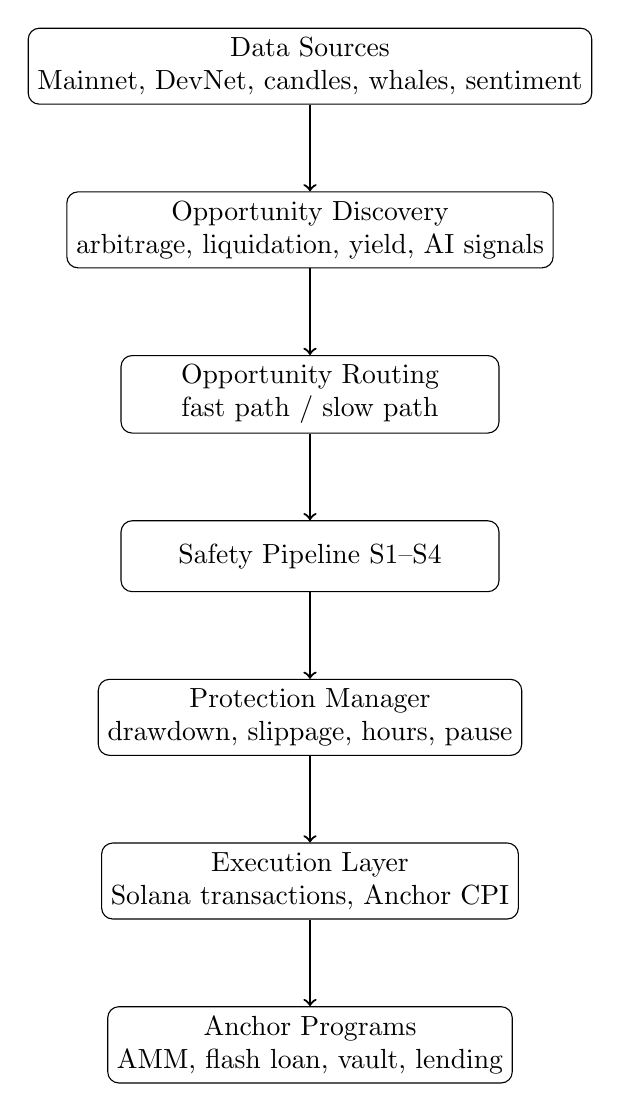
\begin{tikzpicture}[
    node distance=1.1cm,
    box/.style={rectangle, draw, rounded corners, align=center, minimum width=4.8cm, minimum height=0.9cm},
    arrow/.style={->, thick}
]
\node[box] (data) {Data Sources\\Mainnet, DevNet, candles, whales, sentiment};
\node[box, below=of data] (discovery) {Opportunity Discovery\\arbitrage, liquidation, yield, AI signals};
\node[box, below=of discovery] (routing) {Opportunity Routing\\fast path / slow path};
\node[box, below=of routing] (safety) {Safety Pipeline S1--S4};
\node[box, below=of safety] (protection) {Protection Manager\\drawdown, slippage, hours, pause};
\node[box, below=of protection] (execution) {Execution Layer\\Solana transactions, Anchor CPI};
\node[box, below=of execution] (chain) {Anchor Programs\\AMM, flash loan, vault, lending};

\draw[arrow] (data) -- (discovery);
\draw[arrow] (discovery) -- (routing);
\draw[arrow] (routing) -- (safety);
\draw[arrow] (safety) -- (protection);
\draw[arrow] (protection) -- (execution);
\draw[arrow] (execution) -- (chain);
\end{tikzpicture}
\caption{Global system architecture}
\label{fig:architecture}
\end{figure}

\section{Technology Choices}

\begin{table}[H]
\centering
\begin{tabularx}{\textwidth}{lX}
\toprule
\textbf{Technology} & \textbf{Role in the project} \\
\midrule
TypeScript & Backend, trading engine, API, orchestration, and transaction building. \\
Python & AI server, prediction endpoints, and sentiment analysis. \\
Anchor & Development framework for Solana programs. \\
Solana DevNet & On-chain execution and testing environment. \\
Redis & Cache for signals, scores, temporary data, and fast state. \\
LangGraph & Event-driven graph orchestration. \\
React & User dashboard and bot configuration interface. \\
WebSocket & Real-time status and event streaming. \\
\bottomrule
\end{tabularx}
\caption{Technology choices}
\label{tab:technologies}
\end{table}

\section{Graph-Based Orchestration}

An important evolution of the project is the transition from a classical sequential loop to graph-based orchestration. Incoming events are inserted into a per-user queue and consumed by a \texttt{UserLane}. Depending on the event type, the graph activates the appropriate nodes.

The main events are:
\begin{itemize}
    \item \texttt{signals\_timer}: triggers full discovery;
    \item \texttt{arb\_opportunity}: directly sends an arbitrage opportunity;
    \item \texttt{liq\_opportunity}: sends a liquidation opportunity;
    \item \texttt{candle\_closed}: refreshes candle-related signals;
    \item \texttt{mempool\_pressure}: indicates high activity pressure.
\end{itemize}

\section{Fast Path and Slow Path}

The fast path is designed to minimize latency. It mainly concerns arbitrage and liquidation opportunities. These opportunities are already structured when they enter the graph and quickly move toward protection checks and execution.

The slow path concerns opportunities requiring more decision logic, especially AI-driven signals and yield opportunities. It goes through the \texttt{DecisionModel}, confidence thresholds, the safety pipeline, and protection rules before execution.

\section{Multi-User Architecture}

The multi-user platform relies on logical separation by user. Each user has:
\begin{itemize}
    \item a strategy configuration;
    \item a bounded event queue;
    \item a protection state;
    \item an associated vault;
    \item a status stream exposed through API and WebSocket.
\end{itemize}

This separation prevents one user from blocking others. It also makes it easier to apply personalized limits, such as maximum capital per trade or minimum AI score.

\section{Conclusion}

The global architecture relies on layered separation and event-driven orchestration. This organization improves maintainability and makes it possible to adapt the verification level to the opportunity type.

% =========================================================
% Chapter 5
% =========================================================
\chapter{Design and Implementation}
\label{chap:implementation}
\rhead{Design and Implementation}

\section{Introduction}

This chapter details the main system components. It presents the detectors, router, safety pipeline, protection manager, execution layer, Anchor programs, and multi-user platform.

\section{Opportunity Discovery}

The \texttt{Opportunity Discovery} layer transforms raw data into candidate opportunities. It includes two families of detectors: deterministic detectors and detectors based on AI signals.

\subsection{Arbitrage Detector}

The arbitrage detector reads AMM pool reserves and simulates swap cycles. For each cycle, it estimates the output amount after fees and compares it with the input amount.

The simplified profitability condition is:

\begin{equation}
    P_{net} = A_{out} - A_{in} - F_{network} - F_{protocol}
\end{equation}

where $P_{net}$ is the net profit, $A_{out}$ is the obtained amount, $A_{in}$ is the initial amount, $F_{network}$ represents network fees, and $F_{protocol}$ represents swap-related fees.

\subsection{Liquidation Detector}

The liquidation detector observes positions from the lending program. When a position becomes undercollateralized, an opportunity is generated. The DevNet implementation uses a dedicated Anchor program that registers positions and liquidates them according to a health threshold.

\subsection{Yield Detector}

The yield detector compares available rates and generates opportunities when the expected return exceeds a threshold. In the current state, this component remains extensible and can be connected to external yield sources.

\section{Opportunity Routing}

The router is an important decision point. It does not decide whether an opportunity is profitable, but determines the execution path it should follow. Arbitrage and liquidation opportunities are routed to the fast path, while directional, sentiment, whale, or yield opportunities go through the slow path.

\begin{lstlisting}[language=JavaScript, caption={Simplified routing principle}]
if (opportunity.type === "arb" || opportunity.type === "liq") {
  return "fast";
}

if (opportunity.requiresAiScore || opportunity.usesUserCapital) {
  return "slow";
}
\end{lstlisting}

\section{Safety Pipeline S1--S4}

The safety pipeline is applied before risky executions. It is structured into four levels in order to combine explicit rules, simulations, and anomaly detection.

\subsection{S1: On-Chain Heuristics}

The first level checks simple but important properties: mint authority, token distribution, age, possible concentration, and metadata consistency. These rules make it possible to quickly reject obviously dangerous tokens.

\subsection{S2: Honeypot Detection}

The second level aims to detect situations where entering a position is possible but exiting is impossible or heavily penalized. The logic relies on a sell simulation or on the verification of an existing exit path.

\subsection{S3: Isolation Forest}

The third level uses anomaly detection. The objective is to identify unusual behavior that is not necessarily captured by explicit rules. Scores can be cached to reduce latency.

\subsection{S4: Additional Controls}

The final level aggregates additional checks, such as wash trading patterns, abnormal holder variations, or other suspicious indicators.

\section{Protection Manager}

The \texttt{ProtectionManager} applies global rules that are independent from the opportunity type. It acts as a final barrier before execution.

\begin{table}[H]
\centering
\begin{tabularx}{\textwidth}{lX}
\toprule
\textbf{Module} & \textbf{Role} \\
\midrule
Daily Drawdown & Stop or limit trading after a daily loss. \\
Slippage Guard & Prevent a transaction if slippage exceeds the authorized threshold. \\
Trading Hours & Allow trading only during configured time windows. \\
Auto Pause & Pause the bot after several consecutive failures. \\
Vault Check & Verify that the user vault is active and sufficiently funded. \\
\bottomrule
\end{tabularx}
\caption{Protection Manager modules}
\end{table}

\section{Execution Layer}

The execution layer builds Solana transactions. It must integrate the required accounts, Anchor instructions, fees, and atomicity constraints.

\subsection{Flash Loan Arbitrage Transaction}

In the case of arbitrage, the transaction contains several instructions in a strict order. The flash loan program verifies that repayment is present in the same transaction. This constraint prevents a loan from remaining open.

\subsection{Transaction Using the User Vault}

For the slow path, capital must not freely transit through the bot wallet. The user vault, represented by a PDA, acts as the transfer authority. This design improves fund isolation.

\section{Anchor Programs}

\subsection{AMM Program}

The AMM program implements swap and liquidity management operations. It serves as a controlled environment for testing strategies on DevNet.

\subsection{Flash Loan Program}

The flash loan program provides borrow and repay instructions. It enforces atomicity through the structure of the transaction.

\subsection{Vault Program}

The vault program manages deposits, withdrawals, and bot-authorized operations. Each user has a dedicated PDA.

\subsection{Lending Program}

The lending program makes it possible to create loan positions and test honest liquidations. It provides a DevNet framework for validating the liquidation path without depending on an external protocol.

\section{API and WebSockets}

The backend exposes routes to create users, update their configuration, start or stop their engine, and consult their status. WebSockets stream important events, including ticks, opportunities, rejections, and executions.

\section{Conclusion}

The implementation relies on a strict separation between detection, routing, safety, protection, and execution. This separation makes it possible to modify a strategy without compromising the entire system.

% =========================================================
% Chapter 6
% =========================================================
\chapter{Artificial Intelligence and Decision Model}
\label{chap:ai}
\rhead{Artificial Intelligence}

\section{Introduction}

This chapter presents the role of artificial intelligence in the system. The objective is not to replace safety rules or profitability calculations, but to provide complementary signals that better control slow-path decisions.

\section{AI Server}

The AI server is developed in Python. It exposes endpoints consumed by the TypeScript backend. This separation keeps machine learning dependencies outside the main engine and allows models to evolve without modifying the execution layer.

The endpoints mainly cover:
\begin{itemize}
    \item market regime prediction;
    \item direction estimation;
    \item sentiment analysis;
    \item volatility expansion.
\end{itemize}

\section{Data Used}

AI signals combine on-chain and off-chain sources. On-chain data includes wallet movements, pool variations, and certain network events. Off-chain data includes market candles, social or textual information, and price indicators.

\section{Features and Labels}

Possible features include:
\begin{itemize}
    \item short-term returns;
    \item realized volatility;
    \item volume variation;
    \item whale accumulation or distribution;
    \item sentiment score;
    \item mempool pressure;
    \item regime indicators.
\end{itemize}

Labels depend on the task. For directional prediction, the label may represent future price increase or decrease. For volatility, it may represent significant expansion over a given time window.

\section{DecisionModel}

The \texttt{DecisionModel} combines several signals into a single score. This score is then compared with a configurable threshold. The chosen approach is deliberately cautious: a slow opportunity should not be executed only because one model is optimistic.

A simplified formula can be written as:

\begin{equation}
    Score_{AI} = w_1 S_{sentiment} + w_2 S_{whale} + w_3 S_{direction} + w_4 S_{volatility} + w_5 S_{mempool}
\end{equation}

where $w_i$ represents the weight assigned to each signal.

\section{Ablation and Comparison}

To measure the real contribution of AI, several configurations should be compared:
\begin{itemize}
    \item execution without AI;
    \item sentiment only;
    \item whale signals only;
    \item direction only;
    \item complete fusion through \texttt{DecisionModel}.
\end{itemize}

This comparison avoids overestimating the usefulness of the models. It also helps identify which signals truly improve decision quality.

\section{Model Limitations}

AI models applied to trading face several limitations:
\begin{itemize}
    \item financial data is noisy;
    \item market regimes change quickly;
    \item a model can overfit non-generalizable patterns;
    \item social signals can be manipulated;
    \item a good prediction does not guarantee good execution.
\end{itemize}

These limitations justify the use of thresholds, protections, and ablation studies.

\section{Conclusion}

AI is integrated as a decision-support layer. It enriches the available signals, but remains constrained by safety rules, profitability requirements, and system protections.

% =========================================================
% Chapter 7
% =========================================================
\chapter{Experimentation, Results, and Discussion}
\label{chap:evaluation}
\rhead{Experimentation and Discussion}

\section{Introduction}

This chapter presents the experimental environment, evaluation metrics, tests performed, and a discussion of expected or observed results. The objective is to verify not only potential profitability, but also system robustness.

\section{Experimental Environment}

Tests are mainly performed on Solana DevNet. This environment makes it possible to deploy Anchor programs, create test tokens, configure AMM pools, and simulate opportunities without risking real capital.

The system also uses mainnet data for certain signals, especially market data, whale activity, or sentiment, while execution remains limited to DevNet.

\section{Test Scenarios}

The main scenarios studied are:
\begin{enumerate}
    \item creation of a price gap between pools and arbitrage detection;
    \item execution of atomic arbitrage with a flash loan;
    \item rejection of a token marked as risky;
    \item triggering of a slippage limit;
    \item triggering of auto-pause after failures;
    \item liquidation of an undercollateralized position;
    \item propagation of a user configuration to the engine.
\end{enumerate}

\section{Metrics}

\begin{table}[H]
\centering
\begin{tabularx}{\textwidth}{lX}
\toprule
\textbf{Category} & \textbf{Metrics} \\
\midrule
Performance & Tick latency, transaction build time, confirmation time. \\
Opportunity quality & Net profit after fees, executed opportunity rate, rejected opportunity rate. \\
Safety & Number of S1--S4 rejections, false positives, false negatives on injected cases. \\
Stability & Auto-pause triggers, drawdown compliance, queue behavior. \\
AI & Average score, acceptance rate by threshold, comparison with ablations. \\
\bottomrule
\end{tabularx}
\caption{Evaluation metrics}
\end{table}

\section{Unit and Integration Tests}

The project contains several unit and integration tests covering detectors, safety, protection, graph topology, flash loan execution, vault logic, and liquidation. These tests validate components in isolation and then through a more complete flow.

End-to-end tests verify that the pipeline can detect an opportunity, route it, apply checks, and build a coherent transaction.

\section{Discussion}

The resulting architecture shows that it is possible to structure an on-chain trading system into independent layers. This separation improves maintainability and reduces the risk that an error in a detector directly causes capital loss.

The fast path is adapted to opportunities where speed and atomicity are priorities. The slow path, on the other hand, allows additional signals and protections before user capital is used. This distinction is important because not all opportunities have the same risk profile.

The main limitations concern production deployment. DevNet does not fully reproduce mainnet competition, MEV, real liquidity depth, or RPC variability. In addition, AI models must be evaluated on broader data to measure their generalization ability.

\section{Conclusion}

The experiments validate the coherence of the architecture and the feasibility of a complete DevNet pipeline. However, migration to MainNet requires significant hardening: stronger MEV protection, advanced monitoring, strict key management, alerting, and deeper model validation.

% =========================================================
% General conclusion
% =========================================================
\chapter*{General Conclusion}
\addcontentsline{toc}{chapter}{General Conclusion}
\rhead{General Conclusion}

This project focused on the design and implementation of an on-chain trading platform on Solana. The developed system combines several dimensions: opportunity detection, fast path and slow path routing, multi-level safety, capital protection, atomic execution, Anchor smart contracts, artificial intelligence signals, and multi-user architecture.

The work demonstrates the importance of modular architecture in a domain as sensitive as automated trading. The separation between discovery, safety, protection, and execution helps control decisions and reduce the risk of uncontrolled execution. The use of DevNet made it possible to test on-chain mechanisms without exposing real capital.

The Anchor programs provide an experimental basis for swaps, flash loans, vaults, and liquidations. The TypeScript backend orchestrates the components and exposes a multi-user API. The AI server complements decision-making by providing sentiment, volatility, direction, and whale-activity signals.

Nevertheless, several limitations remain. MainNet deployment requires more advanced handling of MEV, RPC quality, real liquidity depth, and operational security. AI models must also be rigorously evaluated to avoid excessive confidence in unstable signals.

The main perspectives are:
\begin{itemize}
    \item connect execution to real aggregators such as Jupiter;
    \item strengthen MEV protection and transaction submission strategy;
    \item improve monitoring, alerting, and dashboards;
    \item perform complete ablation studies of AI signals;
    \item harden vault management and user limits;
    \item explore an agentic layer for analysis and configuration assistance.
\end{itemize}

Thus, this project provides a solid foundation for a more complete on-chain trading platform, while highlighting the level of caution required before any use in a real trading environment.

% =========================================================
% Appendices
% =========================================================
\begin{appendices}

\chapter{Configuration Extract}

\begin{lstlisting}[caption={Example of strategy parameters}]
protection:
  max_consecutive_failures: 3
  drawdown_pause_pct: 5
  slippage_max_bps: 100

capital:
  daily_limit_usd: 100
  flash_loan_max_usd: 1000

ai:
  enabled: true
  min_score: 0.65
\end{lstlisting}

\chapter{Pipeline Pseudo-Code}

\begin{lstlisting}[language=JavaScript, caption={Simplified pipeline}]
async function processOpportunity(opportunity) {
  const route = router.route(opportunity);

  if (route === "slow") {
    const aiScore = await decisionModel.computeScore(opportunity);
    if (aiScore < userConfig.aiThreshold) return "rejected_ai";
  }

  const safety = await safetyPipeline.check(opportunity);
  if (!safety.accepted) return "rejected_safety";

  const guard = await protectionManager.check(opportunity);
  if (!guard.accepted) return "rejected_protection";

  const tx = await transactionBuilder.build(opportunity, route);
  return txSubmitter.submit(tx);
}
\end{lstlisting}

\chapter{Example Results Table}

\begin{table}[H]
\centering
\begin{tabular}{lccc}
\toprule
\textbf{Scenario} & \textbf{Success} & \textbf{Average latency} & \textbf{Comment} \\
\midrule
DevNet arbitrage & To be completed & To be completed & Atomic transaction \\
Liquidation & To be completed & To be completed & Lending program \\
AI slow path & To be completed & To be completed & Depends on AI threshold \\
Safety S1--S4 & To be completed & To be completed & Injected cases \\
\bottomrule
\end{tabular}
\caption{Template for experimental results}
\end{table}

\end{appendices}

\begin{thebibliography}{9}

\bibitem{talanWho}
Talan, \textit{Who We Are}. Available online: \url{https://www.talan.com/americas/en/about-us/our-vision/who-we-are}

\bibitem{talanSummer}
Talan, \textit{Innovation Factory / SummerCamp internship description}. Available online: \url{https://www.talan.com/americas/en/careers/offers/detail/744000058858050}

\bibitem{solana}
Solana Foundation, \textit{Solana Documentation}. Available online: \url{https://solana.com/docs}

\bibitem{anchor}
Coral, \textit{Anchor Framework Documentation}. Available online: \url{https://www.anchor-lang.com/}

\bibitem{defi}
Schär, F., \textit{Decentralized Finance: On Blockchain- and Smart Contract-Based Financial Markets}, Federal Reserve Bank of St. Louis Review, 2021.

\bibitem{flashloans}
Qin, K., Zhou, L., Gervais, A., \textit{Attacking the DeFi Ecosystem with Flash Loans for Fun and Profit}, Financial Cryptography and Data Security, 2021.

\bibitem{mev}
Daian, P. et al., \textit{Flash Boys 2.0: Frontrunning, Transaction Reordering, and Consensus Instability in Decentralized Exchanges}, IEEE Symposium on Security and Privacy, 2020.

\bibitem{isolationforest}
Liu, F. T., Ting, K. M., Zhou, Z.-H., \textit{Isolation Forest}, IEEE International Conference on Data Mining, 2008.

\end{thebibliography}

\end{document}
